\chapter{O Sol no céu: dias e estações}\label{ch:g3:sun-days-seasons}

Em junho você brinca na rua depois do jantar, com uma \omterm{def:g1:light-and-shadows:source}{luz} dourada; em
dezembro os postes acendem antes de você chegar da escola. O Sol
mantém o velho hábito dele --- sobe por um lado, passa pelo alto,
desce pelo outro --- mas a estrada dele pelo céu não é a mesma
estrada o ano inteiro. Acompanhe o Sol durante um ano inteiro e você
descobre as \omterm{def:g3:sun-days-seasons:year}{estações}.

\section{A estrada mutante do Sol}

\begin{example}[Estrada de verão, estrada de inverno]\label{ex:g3:sun-days-seasons:roads}
Observe o arco do Sol no auge do verão: ele nasce cedo, sobe muito
alto --- quase em cima da nossa cabeça ao meio-dia --- e se põe
tarde: uma estrada comprida e alta, e um dia comprido. No auge do
inverno, o arco é baixo e curto: o Sol nasce tarde, nunca sobe muito
acima dos telhados e se põe no meio da tarde. Entre os dois, na
primavera e no outono, a estrada é intermediária --- e o dia e a
noite dividem as \omterm{ex:g2:measuring-time:clock}{horas} quase por igual.
\end{example}

\begin{omfigure}
\begin{tikzpicture}[scale=0.85]
  \draw[thick] (0,0) -- (11,0);
  \draw[dashed, omThm, thick] (1.0,0.2) .. controls (3.5,4.6)
    and (7.5,4.6) .. (10.0,0.2);
  \fill[omThm] (5.5,3.5) circle (0.3);
  \node[above, font=\small, omThm] at (5.5,3.9) {auge do verão: alta e longa};
  \draw[dashed, omDef, thick] (2.6,0.15) .. controls (4.4,1.7)
    and (6.6,1.7) .. (8.4,0.15);
  \fill[omDef] (5.5,1.3) circle (0.3);
  \node[above, font=\small, omDef] at (2.9,1.35) {auge do inverno: baixa e curta};
\end{tikzpicture}

{\small As duas estradas extremas do Sol sobre o mesmo horizonte. O
arco alto de verão leva muitas \omterm{ex:g2:measuring-time:clock}{horas} para ser percorrido; o arco
baixo de inverno termina no meio da tarde.}
\end{omfigure}

\begin{proposition}[A regra do meio-dia]\label{prop:g3:sun-days-seasons:midday}
Em toda \omterm{def:g3:sun-days-seasons:year}{estação}, o Sol fica mais alto no meio do dia --- e nesse
instante toda \omterm{def:g1:light-and-shadows:shadow}{sombra} está no seu tamanho mais curto do dia e aponta
na mesma direção da \omterm{def:g1:light-and-shadows:shadow}{sombra} de meio-dia de ontem, e da de amanhã. As
\omterm{def:g1:light-and-shadows:shadow}{sombras} de meio-dia são as setas mais confiáveis da natureza.
\end{proposition}

\begin{example}[Ler a estação numa sombra]\label{ex:g3:sun-days-seasons:shadowlength}
O \emph{comprimento} da \omterm{def:g1:light-and-shadows:shadow}{sombra} de meio-dia muda com a \omterm{def:g3:sun-days-seasons:year}{estação}: no
verão, com o Sol quase em cima da cabeça, a \omterm{def:g1:light-and-shadows:shadow}{sombra} de meio-dia de um
poste é um tocozinho curto; no inverno, com o Sol lá embaixo, o mesmo
poste joga uma \omterm{def:g1:light-and-shadows:shadow}{sombra} comprida ao meio-dia. Marque no chão a ponta da
\omterm{def:g1:light-and-shadows:shadow}{sombra} de meio-dia uma vez por mês e as marcas vão andar para lá e
para cá ao longo do ano, como um pêndulo lento.
\end{example}

\section{O relógio de sombra}

\begin{definition}[Relógio de sol]\label{def:g3:sun-days-seasons:sundial}
Um \emph{relógio de sol}\index{relógio de sol} é um relógio feito de
\omterm{def:g1:light-and-shadows:shadow}{sombra}: uma haste ou uma lâmina fincada no sol, com marcas em volta
mostrando onde a \omterm{def:g1:light-and-shadows:shadow}{sombra} cai a cada hora. Conforme o Sol percorre o
arco dele, a \omterm{def:g1:light-and-shadows:shadow}{sombra} varre as marcas --- devagar, em silêncio e sem
uma única peça móvel.
\end{definition}

\begin{method}[Construir um relógio de sombra]\label{met:g3:sun-days-seasons:build}
Numa manhã de sol, num lugar que fique ensolarado o dia inteiro:
\begin{enumerate}
  \item finque uma vareta reta em pé num chão plano (ou coloque-a de
        pé num balde de areia);
  \item a cada hora cheia, marque a ponta da \omterm{def:g1:light-and-shadows:shadow}{sombra} com uma pedrinha
        e escreva a hora na pedrinha com giz;
  \item continue até o fim da tarde.
\end{enumerate}
Amanhã, a \omterm{def:g1:light-and-shadows:shadow}{sombra} vai visitar as suas pedrinhas no horário: a sua
vareta agora diz as \omterm{ex:g2:measuring-time:clock}{horas}. (Por um tempo, pelo menos --- conforme a
\omterm{def:g3:sun-days-seasons:year}{estação} escorrega, as \omterm{def:g1:light-and-shadows:shadow}{sombras} escorregam junto, e as suas pedrinhas
vão aos poucos ficar erradas.)
\end{method}

\begin{omfigure}
\begin{tikzpicture}[scale=0.85]
  \draw[thick] (0.5,0) -- (10.5,0);
  \draw[very thick] (5.5,0) -- (5.5,1.7);
  \draw[line width=3pt, omExo] (5.5,0) -- (2.2,0.9);
  \draw[line width=3pt, omExo, opacity=0.6] (5.5,0) -- (4.1,1.35);
  \draw[line width=3pt, omExo, opacity=0.35] (5.5,0) -- (5.5,1.5);
  \draw[line width=3pt, omExo, opacity=0.6] (5.5,0) -- (6.9,1.35);
  \draw[line width=3pt, omExo] (5.5,0) -- (8.8,0.9);
  \node[font=\footnotesize] at (1.8,1.0) {manhã};
  \node[font=\footnotesize] at (5.5,1.9) {meio-dia: a mais curta};
  \node[font=\footnotesize] at (9.4,1.0) {tarde};
\end{tikzpicture}

{\small Uma vareta, um dia: a \omterm{def:g1:light-and-shadows:shadow}{sombra} varre como um ponteiro lento,
mais comprida nas bordas do dia, mais curta ao meio-dia.}
\end{omfigure}

\section{O ano e as suas estações}

\begin{definition}[O ano e as estações]\label{def:g3:sun-days-seasons:year}
Enquanto a Terra gira uma vez por dia, ela também percorre uma viagem
enorme \emph{em volta do Sol} --- uma volta completa leva um
\emph{ano}\index{ano}, cerca de $365$ dias. Ao longo dessa volta, a
estrada do Sol pelo nosso céu vai subindo e descendo devagar, e nós
passamos pelas quatro \emph{estações}\index{estação}: primavera,
verão, outono, inverno --- e depois primavera de novo, volta após
volta.
\end{definition}

\begin{example}[Os quatro quartos]\label{ex:g3:sun-days-seasons:quarters}
Verão: Sol alto, dias compridos, \omterm{def:g1:light-and-shadows:shadow}{sombras} curtas ao meio-dia. Inverno:
Sol baixo, dias curtos, \omterm{def:g1:light-and-shadows:shadow}{sombras} compridas ao meio-dia. A primavera e
o outono ficam no meio --- e em cada um deles há um dia especial em
que o dia e a noite duram exatamente o mesmo tempo. Os agricultores,
os navegantes e os construtores de antigamente aprenderam a ler esse
calendário direto no céu.
\end{example}

\begin{omfigure}
\begin{tikzpicture}[scale=0.85]
  \fill[omThm] (5.5,1.8) circle (0.5);
  \foreach \a in {0,30,...,330} {
    \draw[omThm] (5.5,1.8) ++(\a:0.68) -- ++(\a:0.26);
  }
  \draw[dashed, thick] (5.5,1.8) ellipse (4.4 and 1.55);
  \fill[omDef] (1.1,1.8) circle (0.26);
  \fill[omDef] (9.9,1.8) circle (0.26);
  \fill[omDef] (5.5,3.35) circle (0.26);
  \fill[omDef] (5.5,0.25) circle (0.26);
  \node[left, font=\small] at (0.75,1.8) {aqui, inverno};
  \node[right, font=\small] at (10.25,1.8) {aqui, verão};
  \node[above, font=\small] at (5.5,3.7) {primavera};
  \node[below, font=\small] at (5.5,-0.1) {outono};
\end{tikzpicture}

{\small Uma volta da Terra em torno do Sol --- um ano, quatro
estações. Por que a estrada baixa no inverno e a estrada alta no
verão? Esse segredo fica guardado para um capítulo mais adiante,
sobre a família Sol--Terra--Lua.}
\end{omfigure}

\begin{remark}[O inverno não é ``mais longe'']\label{rem:g3:sun-days-seasons:notfarther}
É tentador chutar que o inverno é frio porque a Terra se afasta do
Sol. Não é isso --- a distância quase não muda, e, quando é inverno
aqui, é verão para as crianças da outra metade da Terra no mesmíssimo
instante, o que nenhum ``mais longe'' explicaria! A chave de verdade
é a \emph{estrada baixa} do Sol: Sol baixo, \omterm{def:g1:light-and-shadows:source}{luz} inclinada,
aquecimento fraco. A explicação completa fica prometida para um
capítulo mais adiante.
\end{remark}

\begin{omfigure}
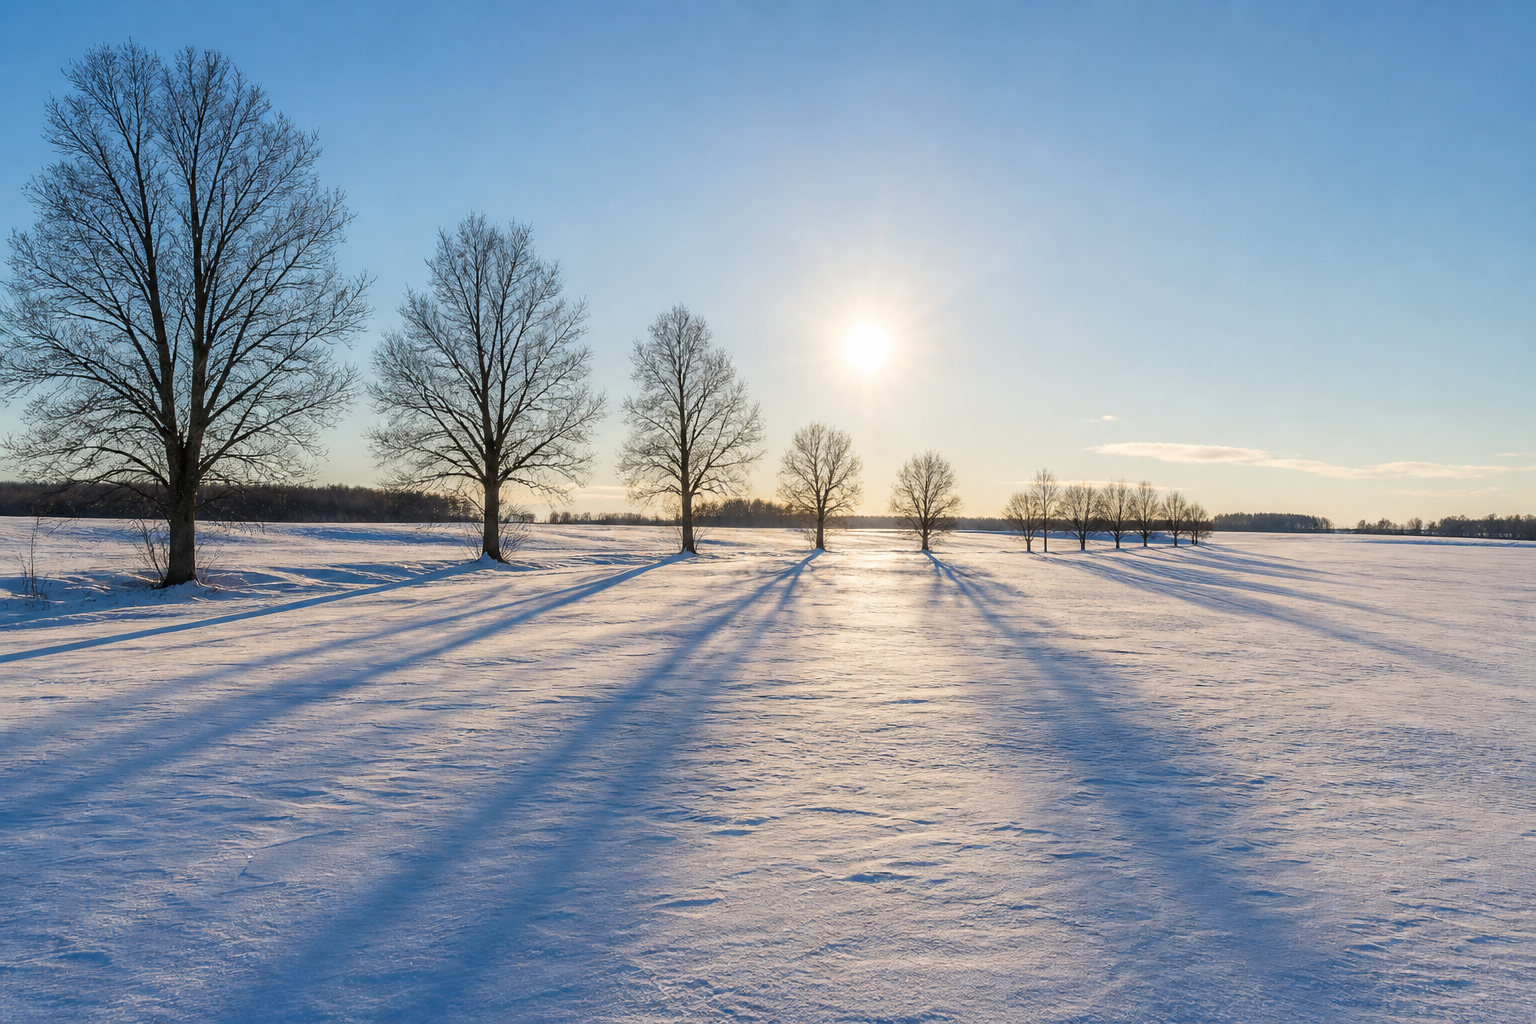
\includegraphics[width=0.58\linewidth]{images/book1/ai/g3-seasons-winter-sun.png}

{\small Um meio-dia de inverno: o Sol fica baixo, a \omterm{def:g1:light-and-shadows:source}{luz} chega inclinada e as \omterm{def:g1:light-and-shadows:shadow}{sombras} se esticam pela neve.}
\end{omfigure}

\section{Exercícios}

\begin{exercise}[$\star$]\label{exo:g3:sun-days-seasons:1}
Em qual \omterm{def:g3:sun-days-seasons:year}{estação} o arco do Sol é o mais alto e o mais comprido? E o
mais baixo e mais curto? O que isso faz com a \omterm{def:g2:measuring-time:duration}{duração} do dia?
\end{exercise}

\begin{exercise}[$\star$]\label{exo:g3:sun-days-seasons:2}
Em que momento do dia a \omterm{def:g1:light-and-shadows:shadow}{sombra} de um poste é a mais curta? O que mais
a \omterm{def:g1:light-and-shadows:shadow}{sombra} de meio-dia tem de especial, dia após dia?
\end{exercise}

\begin{exercise}[$\star$]\label{exo:g3:sun-days-seasons:3}
O mesmo poste joga uma \omterm{def:g1:light-and-shadows:shadow}{sombra} de meio-dia de $2$ botas de comprimento
em junho e de $7$ botas em dezembro. Explique a diferença com as duas
estradas do Sol.
\end{exercise}

\begin{exercise}[$\star$]\label{exo:g3:sun-days-seasons:4}
Como um \omterm{def:g3:sun-days-seasons:sundial}{relógio de sol} diz as \omterm{ex:g2:measuring-time:clock}{horas}? Do que é feito o ponteiro móvel
dele?
\end{exercise}

\begin{exercise}[$\star$]\label{exo:g3:sun-days-seasons:5}
No \cref{met:g3:sun-days-seasons:build}, por que a vareta precisa
ficar num lugar ensolarado o dia inteiro? O que acontece com o
relógio em tempo nublado --- e de noite?
\end{exercise}

\begin{exercise}[$\star$]\label{exo:g3:sun-days-seasons:6}
Quanto tempo a Terra leva para dar uma volta em torno do Sol? Quantas
\omterm{def:g3:sun-days-seasons:year}{estações} cabem numa volta? Ponha-as em ordem, começando pela
primavera.
\end{exercise}

\begin{exercise}[$\star$]\label{exo:g3:sun-days-seasons:7}
Quantos dias tem um ano, mais ou menos? E --- de um capítulo anterior
--- quantas \omterm{ex:g2:measuring-time:clock}{horas} tem um dia? Qual viagem da Terra produz cada um
deles?
\end{exercise}

\begin{exercise}[$\star$]\label{exo:g3:sun-days-seasons:8}
Diga duas pistas, visíveis da sua janela numa única semana, que
mostram se você está no auge do verão ou no auge do inverno, sem
calendário nenhum.
\end{exercise}

\begin{exercise}[$\star$]\label{exo:g3:sun-days-seasons:9}
Quando é inverno onde você mora, que \omterm{def:g3:sun-days-seasons:year}{estação} é para as crianças da
outra metade da Terra? O que isso prova sobre o palpite ``o inverno
acontece porque a Terra inteira está mais longe do Sol''?
\end{exercise}

\begin{exercise}[$\star\star$]\label{exo:g3:sun-days-seasons:10}
Uma jardineira coloca as pedrinhas do relógio de \omterm{def:g1:light-and-shadows:shadow}{sombra} dela em
março. Em junho a \omterm{def:g1:light-and-shadows:shadow}{sombra} não encosta mais nas pedrinhas nas \omterm{ex:g2:measuring-time:clock}{horas}
marcadas. Será que a vareta se mexeu? Explique o que escorregou,
usando o \cref{ex:g3:sun-days-seasons:shadowlength}.
\end{exercise}

\begin{exercise}[$\star\star$]\label{exo:g3:sun-days-seasons:11}
Uma exploradora acorda sem relógio e sem celular, vê o Sol exatamente
no ponto mais alto e, uma hora depois, percebe que a \omterm{def:g1:light-and-shadows:shadow}{sombra} da
barraca dela já está mais comprida que a altura da barraca. Que \omterm{ex:g2:measuring-time:clock}{horas}
eram, mais ou menos, quando ela acordou, e ela está mais perto do
auge do verão ou do auge do inverno? Argumente com a regra do
meio-dia e com o comprimento da \omterm{def:g1:light-and-shadows:shadow}{sombra}.
\end{exercise}
